\RequirePackage[l2tabu, orthodox]{nag}

\documentclass[platex,dvipdfmx]{beamer}			% for platex
\usepackage{graphicx}
\usepackage{bxtexlogo}

%デザインの選択 (省略可)
% \usetheme{default}
\usetheme{Frankfurt}

\title{数値計算のグラフまとめ}

\author{9BSP1118 村岡海人}
\date{\today}

% スライドの始まり
\begin{document}

% タイトルページ
\frame{\maketitle}

% スライド Example
\begin{frame}{スライド}
数式を書くことができるよ。
\begin{equation}
    \frac{1}{s^{2}}\frac{\partial^{2} u}{\partial t^{2}} = \frac{\partial^{2} u}{\partial x^{2}} + \frac{\partial^{2} u}{\partial y^{2}} + \frac{\partial^{2} u}{\partial z^{2}}
\end{equation}
\end{frame}

% 目次ページ
\begin{frame}{目次}
    \tableofcontents
\end{frame}

% 目次の具体例
\section{目次の具体例}
\begin{frame}{スライド}
arrayも使えます.
\begin{align}
    x &= a + 3 \\
    y &= b -4
\end{align}
\end{frame}

% 箇条書き
\section{5量子ビットの時のグラフ}
\begin{frame}{理想的な回数$k$とノイズ$\delta_y$がある時の回数$k_{\text{theory}}$}
    \begin{columns}[onlytextwidth]
        \begin{column}{.45\textwidth}
            5量子ビットの時の理想とノイズのある繰り返し回数の差
        \end{column}
        \hfill
        \begin{column}{.60\textwidth}
        \begin{figure}
          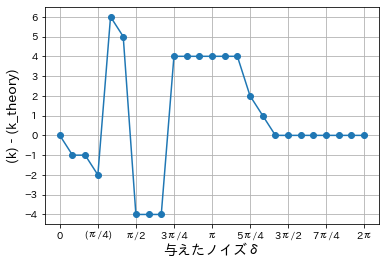
\includegraphics[width=\textwidth]{figures/5qubits/5Qubitk_theory.png}
          \caption{5量子ビットの理想的な回数$k$とノイズ$\delta_y$がある時の回数$k_{\text{theory}}$}
        \end{figure}
        \end{column}
        \end{columns}
\end{frame}

\begin{frame}{理想的な回数$k$の時の解の確率}
    \begin{columns}[onlytextwidth]
        \begin{column}{.45\textwidth}
            5量子ビットの時の理想とノイズのある繰り返し回数の差
        \end{column}
        \hfill
        \begin{column}{.60\textwidth}
        \begin{figure}
            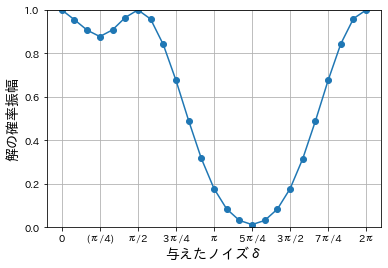
\includegraphics[width=\textwidth]{figures/5qubits/p(k).png}
          \caption{5量子ビット時の解の確率とノイズ$\delta_y$の関係}
        \end{figure}
        \end{column}
        \end{columns}
\end{frame}

% 表スライド
% \section{表}
% \begin{frame}{表の追加}
%     \begin{table}
%         \caption{Caption}
%         \label{table:sample}
%         \centering
%             \begin{tabular}{ccc}
%             \hline
%             料理    & 値段   &  場所  \\
%             \hline \hline
%             チキン  & 200円  & 公園 \\
%             ピザ    & 300円  & 公園 \\
%             ご飯    & 100円  & 室内 \\
%             パン    &  70円  &  室内 \\
%             \hline
%             \end{tabular}
%     \end{table}
% \end{frame}
\end{document}